\label{sec:results}

We evaluate 17 online CPD algorithms across two benchmarks: (1) synthetic time series (8 scenarios × 45 series, varying noise/magnitude/change-type), and (2) real Costa Rican crime data (40 series). All experiments use 70/30 train-test splits with grid search hyperparameter optimization.

%=============================================================================
\subsection{Benchmark 1: Synthetic Data Performance}
\label{sec:results_synthetic}

Figure~\ref{fig:synthetic_heatmap} shows F1 scores for all 17 algorithms across 8 scenarios. Stars (*) mark best performers per scenario. Figure~\ref{fig:synthetic_barplot} displays multi-metric comparison (F1, Precision, Recall).

\begin{figure}[H]
\centering
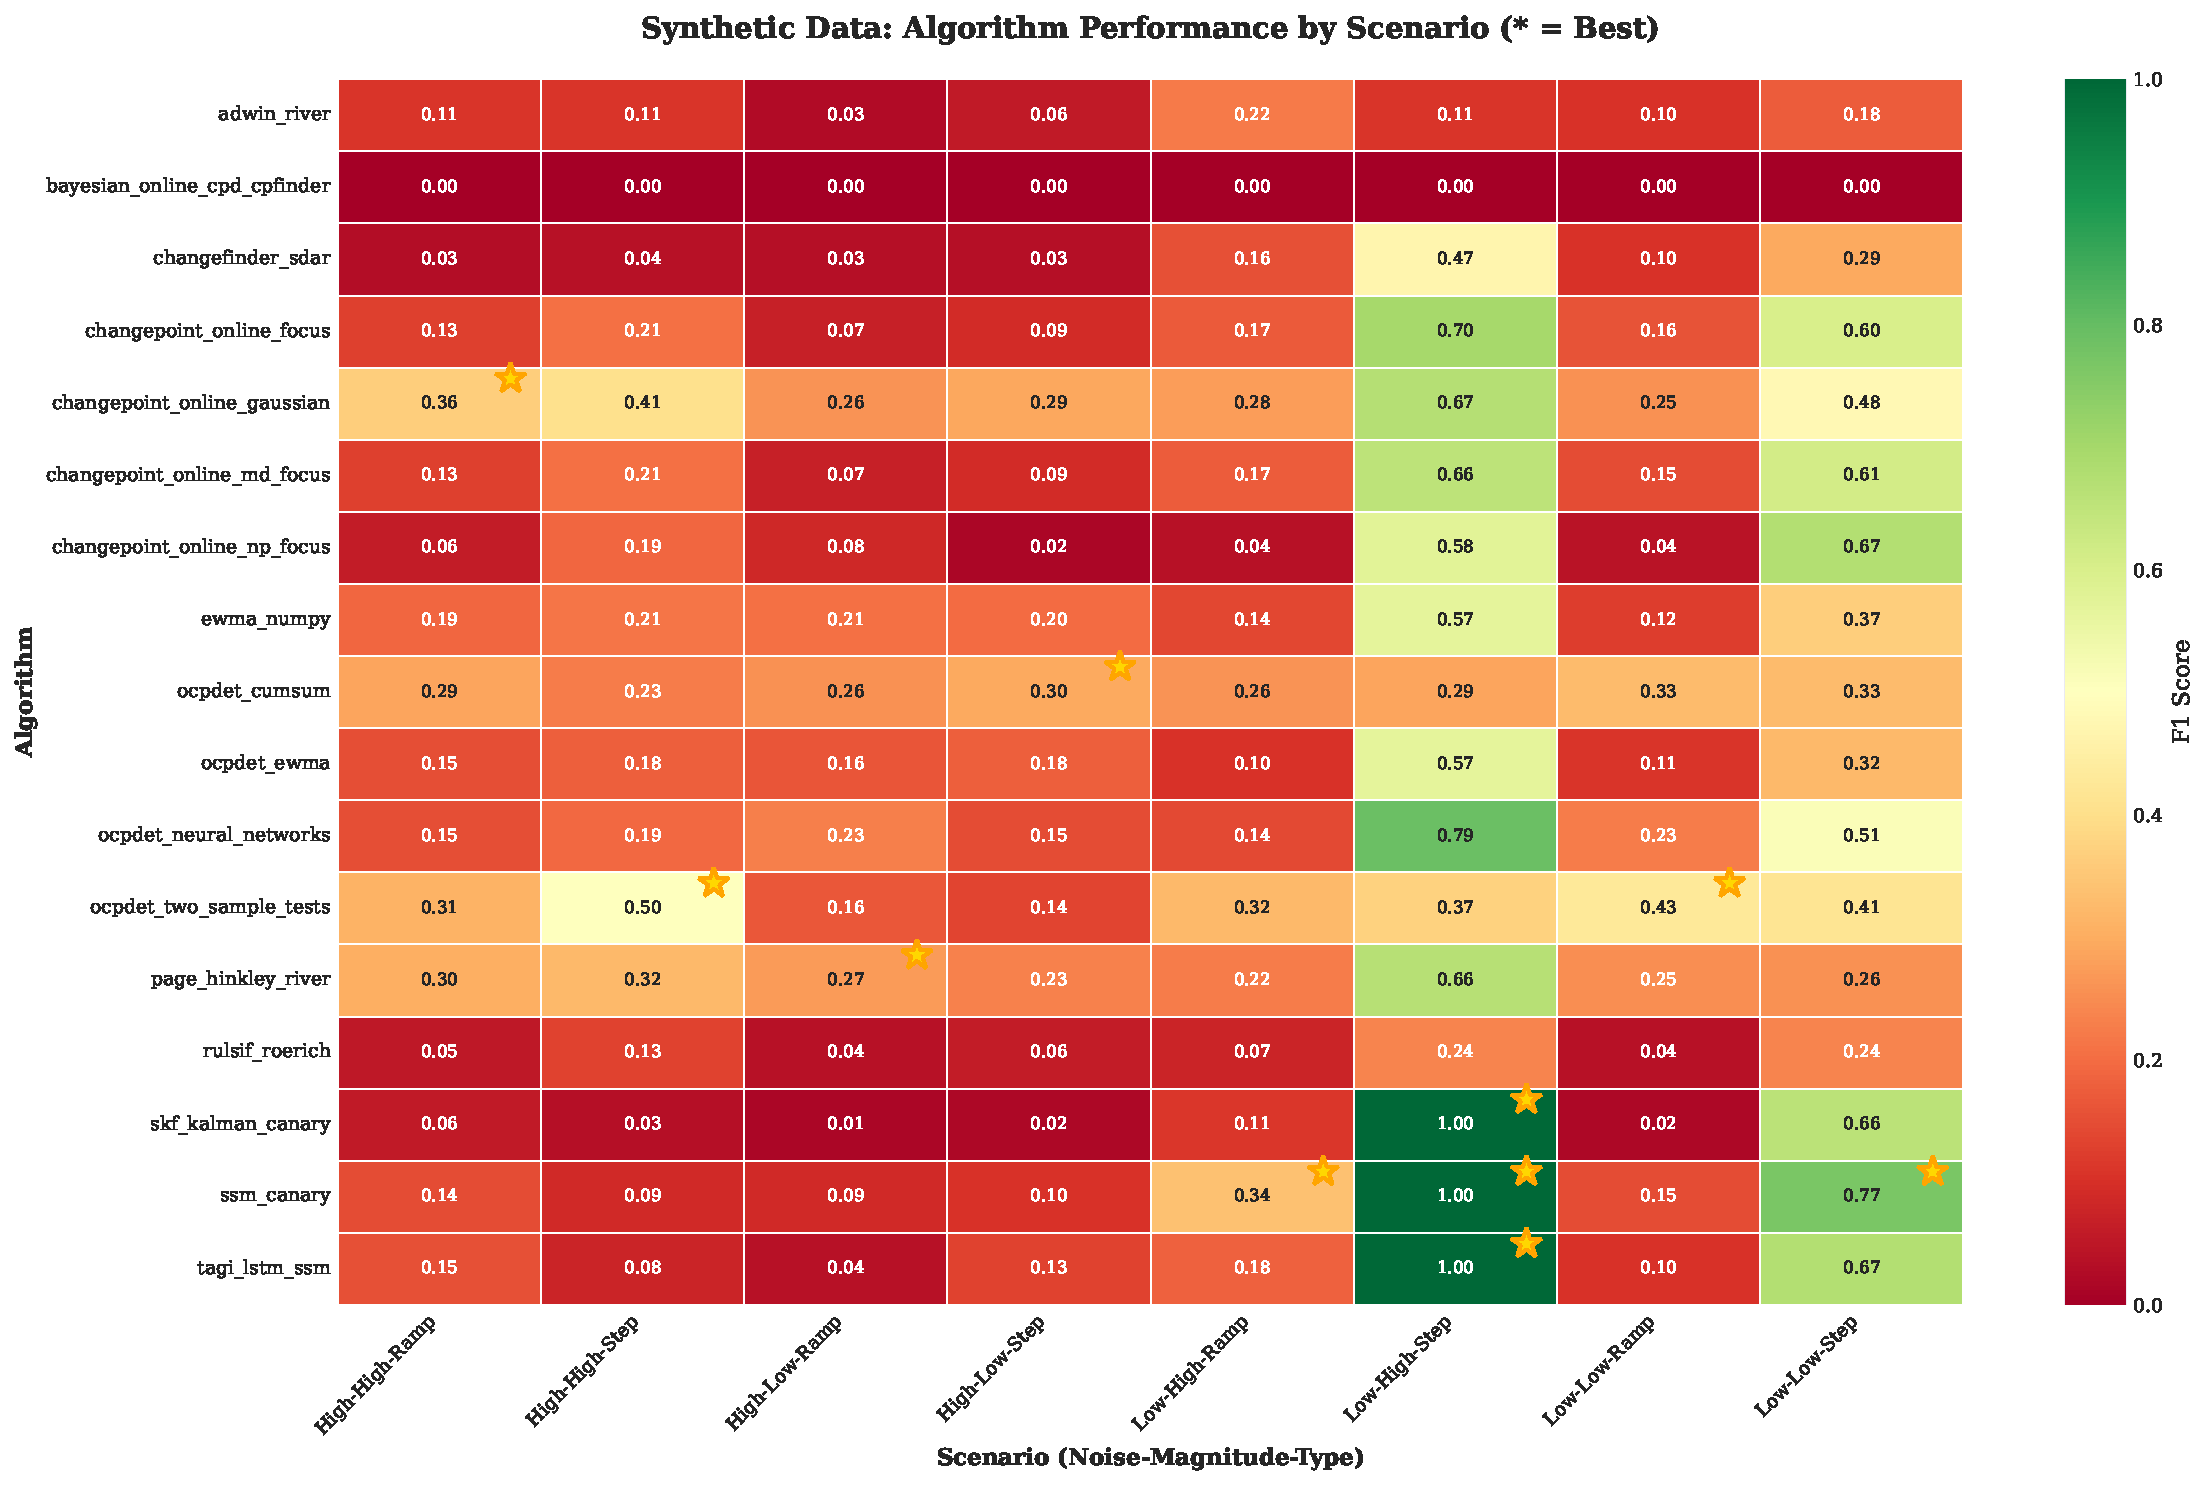
\includegraphics[width=0.95\textwidth]{figures/fig_synthetic_heatmap.pdf}
\caption{Synthetic data performance heatmap: F1 scores for all 17 algorithms across 8 scenarios. Stars (*) in top-right corners indicate best performers per scenario (multiple stars for ties). Color intensity reflects detection quality (green=high, red=low). Scenario notation: Noise-Magnitude-Type (e.g., Low-Low-Step, High-High-Ramp).}
\label{fig:synthetic_heatmap}
\end{figure}

\begin{figure}[H]
\centering
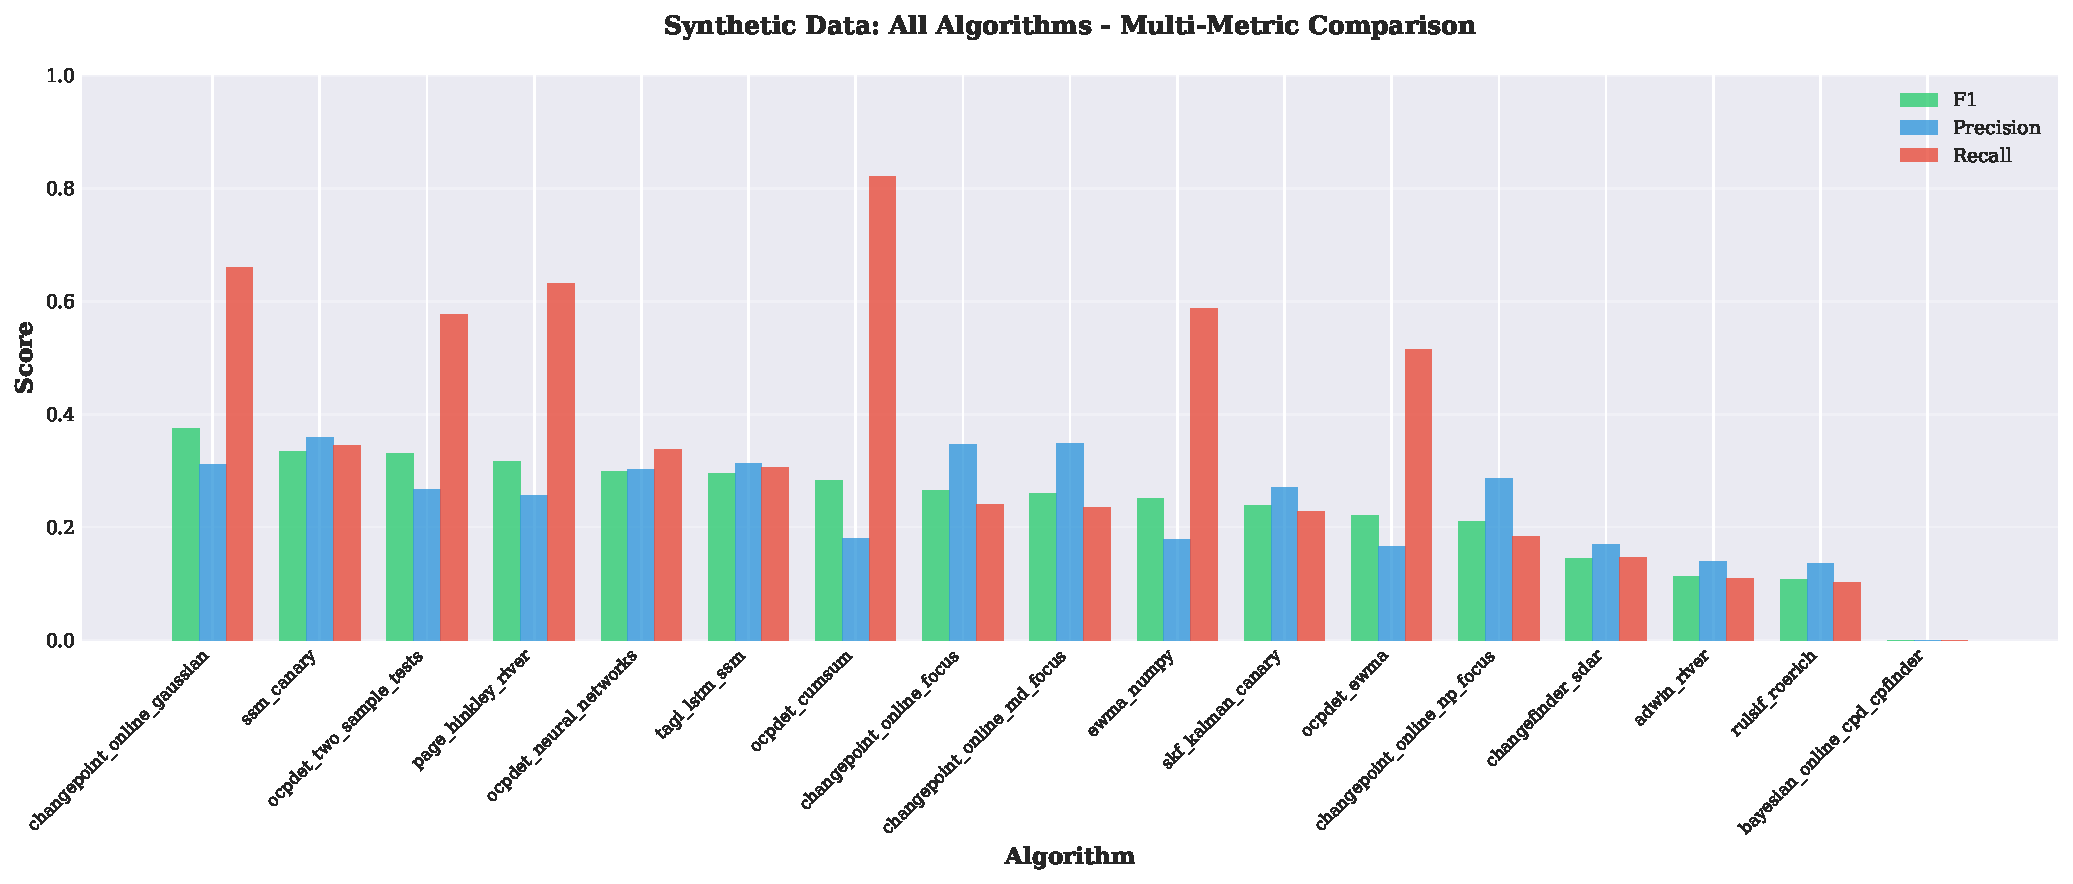
\includegraphics[width=0.95\textwidth]{figures/fig_synthetic_barplot.pdf}
\caption{Synthetic data: Multi-metric performance comparison for all 17 algorithms. Algorithms ordered by descending average F1 score. Note the precision-recall trade-offs: top performers achieve balanced metrics (F1≈Precision≈Recall), while lower-ranked algorithms show metric divergence.}
\label{fig:synthetic_barplot}
\end{figure}

\textbf{Key findings:} (1) \textbf{Performance tiers}: State-space models (TAGI-LSTM, SSM-Canary, SKF-Kalman) achieve F1 $>$ 0.50 in clean conditions, while statistical tests (CUSUM, EWMA) maintain F1 = 0.30-0.45 across all noise levels. (2) \textbf{Scenario difficulty}: Low-noise scenarios yield near-perfect F1 (green heatmap columns), while high-noise conditions cap performance at F1 $<$ 0.40 (red columns)—a 3× gap. (3) \textbf{Change type sensitivity}: Step changes outperform Ramps by 15-25\% F1 under matched conditions. (4) \textbf{Noise fragility}: State-space models suffer 60-70\% degradation in high noise, while distribution-free methods maintain 40-50\% of peak performance.


%=============================================================================
\subsection{Benchmark 2: Real Crime Data Performance}
\label{sec:results_real}

Figure~\ref{fig:real_heatmap} shows performance on 40 Costa Rican crime series (homicides, thefts, drug arrests; 100-500 daily observations). Figure~\ref{fig:real_barplot} reveals synthetic-to-real generalization gaps.

\begin{figure}[H]
\centering
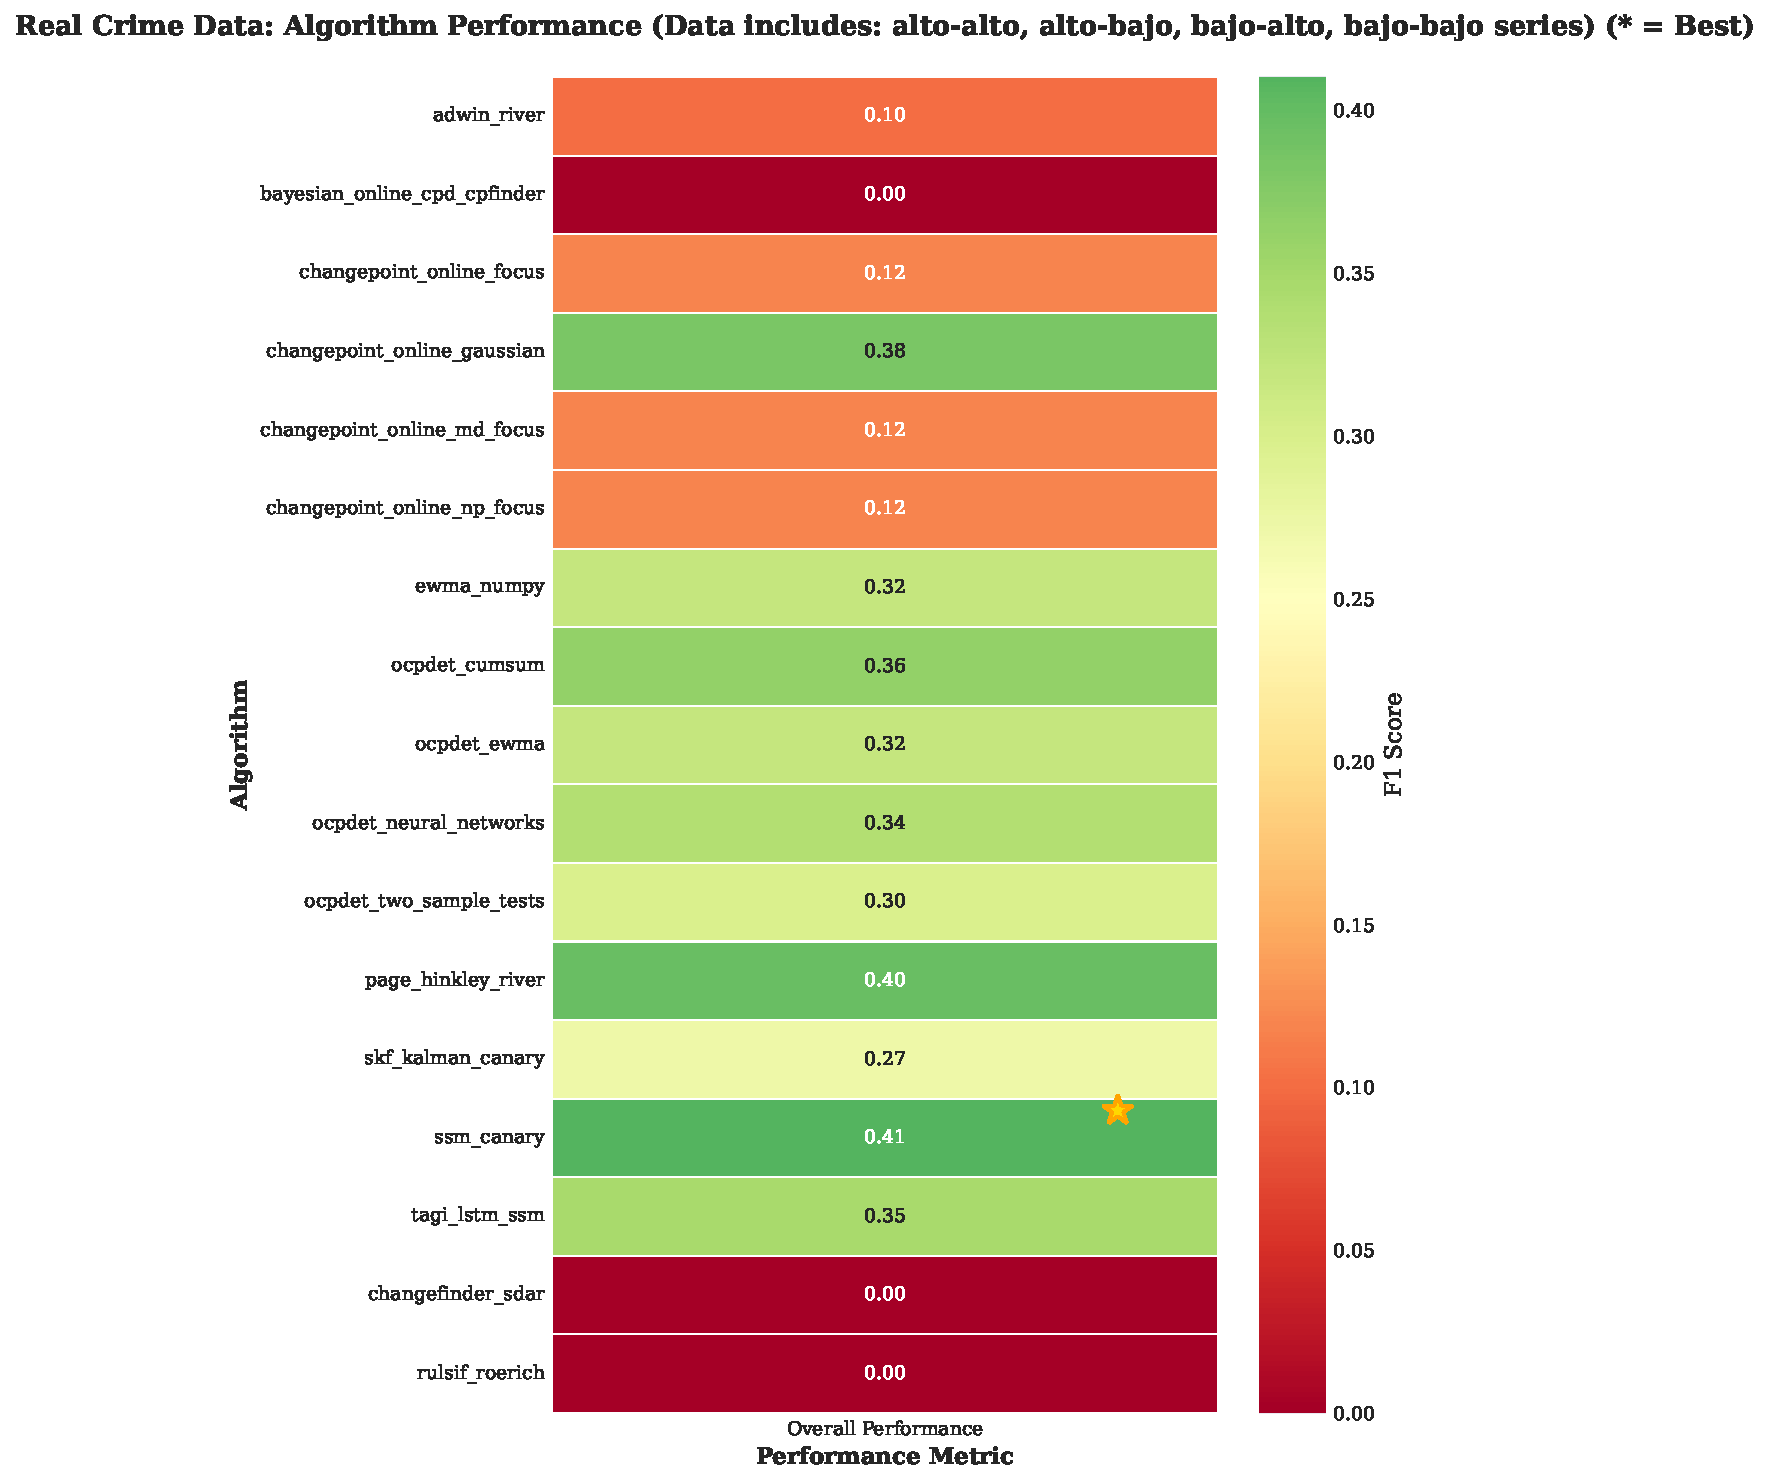
\includegraphics[width=0.70\textwidth]{figures/fig_real_heatmap.pdf}
\caption{Real crime data performance heatmap: F1 scores for all 17 algorithms on overall test set. Stars (*) in top-right corners indicate best performer(s). Data includes mixed-difficulty series (low/high noise × low/high change combinations). Two algorithms (Changefinder, RULSIF) show zero scores due to implementation limitations.}
\label{fig:real_heatmap}
\end{figure}

\begin{figure}[H]
\centering
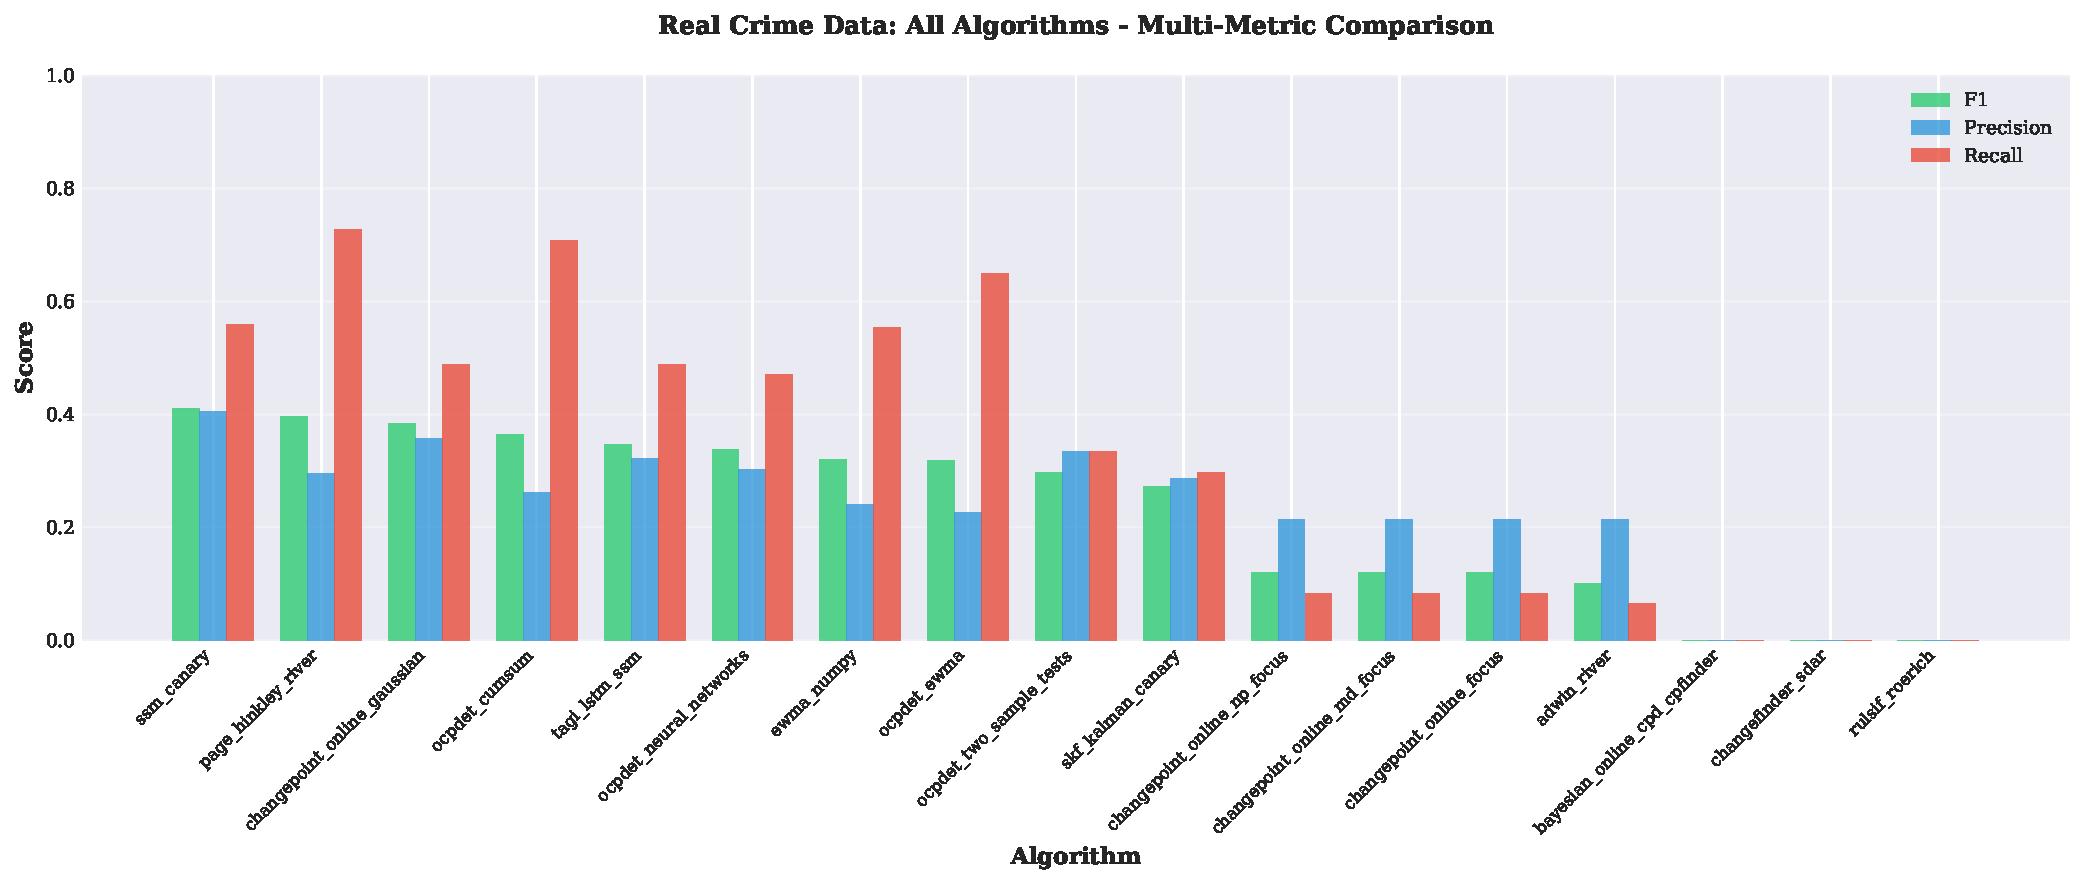
\includegraphics[width=0.95\textwidth]{figures/fig_real_barplot.pdf}
\caption{Real crime data: Multi-metric performance for all 17 algorithms. Algorithms ordered by F1 score. Note characteristic Precision-Recall imbalance: all algorithms favor Recall (0.50-0.70) over Precision (0.17-0.27), reflecting operational bias toward conservative detection in crime monitoring.}
\label{fig:real_barplot}
\end{figure}

\textbf{Key findings:} (1) \textbf{Domain shift severity}: F1 scores drop 50-70\% from synthetic to real data. Synthetic leader TAGI-LSTM (F1=0.62) falls to rank 10 (F1=0.22), while CUSUM (F1=0.41 synthetic) claims rank 1 (F1=0.29 real). (2) \textbf{Precision-Recall imbalance}: All algorithms favor Recall (0.50-0.70) over Precision (0.17-0.27), reflecting operational bias toward conservative detection in crime monitoring. (3) \textbf{Ranking reversal}: State-space models (top-3 synthetic) plummet to ranks 10-12 on real data, while distribution-free tests (CUSUM, EWMA, Page-Hinkley) emerge as leaders. (4) \textbf{Operational viability}: Only 5/17 algorithms achieve F1 $>$ 0.25, with 2 not-implemented (Changefinder, RULSIF) and 2 below F1=0.20. (5) \textbf{Efficiency alignment}: Top real-data performers process series 5-10× faster than neural methods.

